\section{Periodic Motion}

\makelabheader %(Space for student name, etc., defined in master.tex or labmanual_formatting_commands.tex)

\instructornote{%
By Will Hodge, fall 2023.  Updated to use wireless motion and force sensors.
}

\medskip
\textbf{Objectives }
\begin{itemize}[nosep]
\item To learn about some of the characteristics of periodic motion, namely period, frequency, and amplitude. 
\item To investigate the relationships between position, velocity, acceleration, and force in periodic motion. 
\item To investigate energy in simple harmonic motion.
\end{itemize}

\medskip
\textbf{Apparatus} 
\begin{itemize}[nosep]
\item \textit{Capstone} software (\filename{P\_V\_Graphs.cap} and \filename{SHM.cap} experiment files)
\item Spring
\item Support with cross bar
\item Variety of masses 
\item Wireless force sensor
\item Wireless motion sensor 
\end{itemize}

\medskip
\textbf{Introduction }

Periodic motion is motion that repeats itself. You can see the repetition in
graphs of position, velocity, or acceleration vs. time. The length of time to
go through one complete cycle is called the \textit{period}. The
number of cycles in each second is called the \textit{frequency}. The unit of frequency,
cycles per second, is called \textit{Hertz}.

\bigskip
\textbf{Activity 1: Periodic Motion of a Mass-Spring System} 

(a) Open the file \filename{P\_V\_Graphs.cap} in the \filename{\coursefolder} folder. Turn on the motion sensor at your station and connect it to the computer via Bluetooth. Hang the large spring from the force sensor's hook with the large diameter coils down and hang a 200-g mass from the spring.  Place the motion sensor facing up directly below the spring. Lift the mass straight upward about 10~cm, and let go.  You may need to adjust the height of the support for the sensor to see the mass well. Record data for a few seconds to display position-time and 
velocity-time graphs of the motion. Sketch the graphs on the following axes.

%\begin{center}
%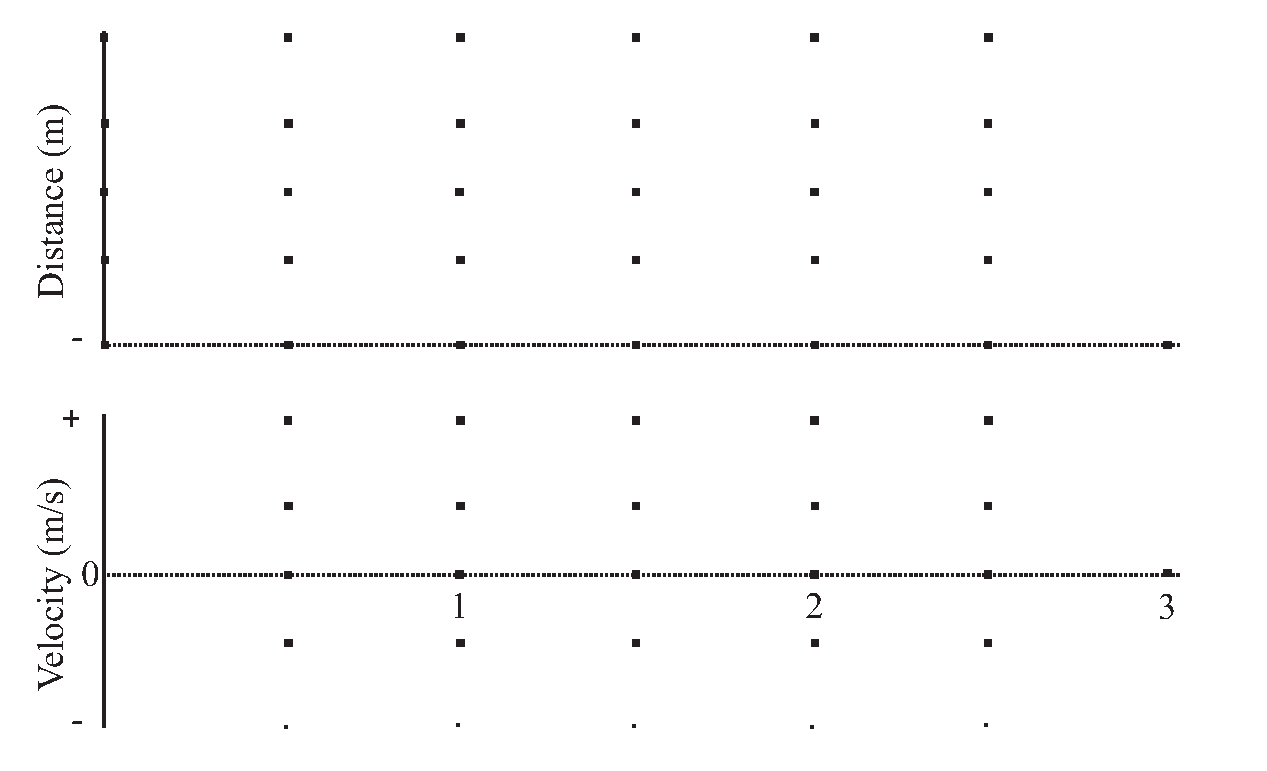
\includegraphics[height=3.5in]{periodic_motion/periodic_motion_fig1_new.eps}
%\end{center}
\begin{lab_groupplot}*{}[lab_grid,
	group style={
		group size=1 by 2,
		xlabels at=edge bottom,
		vertical sep=0.3in,
		},
	width=4.2in,  height=1.4in,
	xlabel=Time (s),
	xmin=0, xmax=3,
	xtick distance = 1, 
	ytick distance = 1, 
	minor x tick num=3,
	minor y tick num=1,
	ytick = {-1,0,1},
	yticklabels = {$-$, 0, $+$},
	]
\nextgroupplot[
	ytick distance = 1, 
	minor y tick num=3,
	ymin=0,ymax=1, 
	ylabel={Position (m)},
	]
\nextgroupplot[
	ymin=-1,ymax=1, 
	ylabel={Velocity (m/s)},
	]
\end{lab_groupplot}

\textit{Note that when an object returns to the same position, it 
does not necessarily mean that a cycle is ending. It must return to the same 
position, and the velocity and acceleration must also return to the same 
values in both magnitude and direction for this to be the start of a new cycle.}

%(b) Label the graphs above with: ``B'' at the Beginning of a
%cycle and ``E'' at the End of the same complete cycle. ``A''
%on each spot where the mass is moving Away from the detector fastest. ``T''
%on each spot where the mass is moving Toward the detector fastest. ``S''
%on each spot where the mass is standing Still. ``F'' where the
%mass is Farthest from the motion detector. ``C'' where the mass
%is Closest to the motion detector.

(b) Do the position and velocity graphs appear to have the same period? Do their
peaks occur at the same times? If not, how are the peaks related in time, i.e. 
what fraction of a period is their phase difference?
\vspace{20mm}

(c) Use the \textbf{Delta Tool} to measure the period of the motion. (For
better accuracy, measure the total time over as many cycles as possible and
divide by the number of cycles.)
\vspace{20mm}

(d) Using the \textbf{Statistics} function, determine and record the maximum and minimum 
displacement.  Determine the amplitude of the motion from $A = (x_{\rm max} - x_{\rm min})/2$.
\vspace{20mm}

(e) Save the graph. You will be using it again in Activity 5.

\bigskip

\textbf{Activity 2: Predictions:  What Factors Determine the Period of the Mass-Spring System? }

The motion of a mass hanging from a spring that you looked at in Activity 1
is a close approximation to a kind of periodic motion called simple harmonic
motion (abbreviated SHM).

(a) What can you do to change the period of the SHM of the mass-spring system? What
will happen to the period if you increase the amplitude? Increase the mass?
Increase the spring constant (use a stiffer spring)?
\answerspace{20mm}

(b) Repeat the procedure of Act 1, but with a different starting position
(other than 10~cm). (Warning: Do not make the amplitude so large that the mass
comes closer than 15~cm from the motion sensor.) When you have good graphs,
find and record the period and the amplitude using the methods described in
Activity 1. 
\answerspace{15mm}

%(b) Take ratios of the period and the amplitude of Activity 1 to those 
%determined here.
%\vspace{20mm}

(c) Is there evidence that the period depends on amplitude? (Did the change
in amplitude result in a comparable change in period?) How does this
compare with your prediction?
\answerspace{10mm}

\pagebreak[2]
(d) Carefully measure the period for four other masses. Record the masses and
the measured periods in a table in the space below along with the mass and 
period from Activity 1. %\textbf{Note:} Add half the mass of the spring to each mass value. This accounts for the fact that the theory of SHM neglects the mass of the spring.
\textbf{Note:} Add one third of the mass of the spring to each mass value. This accounts for the fact that the theory of SHM neglects the mass of the spring.
\answerspace{35mm}

(e) Does the period depend on the mass? Does it increase or decrease as mass
is increased?
\answerspace{15mm}

(f) Determine the mathematical relationship between the period $T$ and the mass
$m$ by finding a function that fits the data. Do this by using \textit{Excel} to plot 
a graph of $T$ vs. $m$ (%use the TOTAL mass including half the mass of the 
use the total mass, including one third of the mass of the spring) and fitting the data with a POWER function. Write the equation that provides the best fit to the data in the space below. What is the power of $m$ for your best fit? Print the graph and include with this unit.
\answerspace{20mm}

You should have found that $T$ is independent of amplitude 
and proportional to \( \sqrt{m} \). The actual expression for the period is
\[T=2\pi \sqrt{\frac{m}{k}.}\]


%\textbf{Velocity, Acceleration, Force and Energy }
%
%In this investigation you will look more carefully at the distance, velocity
%and acceleration graphs for simple harmonic motion. You will also look at the
%force graph, and will examine the energy associated with simple harmonic motion.

\textbf{Activity 3: Determination of the Spring Constant }

Measure the distance the spring stretches for four different masses and use
these data to determine the spring constant, $k$, as you did in either the Work and Kinetic Energy experiment or the Hooke's Law experiment. Record your data and the result for $k$ in the space below.
\answerspace{40mm}

\pagebreak[2]
\textbf{Activity 4: Velocity, Acceleration, and Force for SHM} 

(a) Consider the motion you looked at in Activity 1 when the mass was 200 g
and the initial position was 10~cm. Sketch the position and velocity graphs
that you observed on the axes below using dashed lines.

%\vspace{0.3cm}
%\begin{center}
%\hspace{0.15in}
%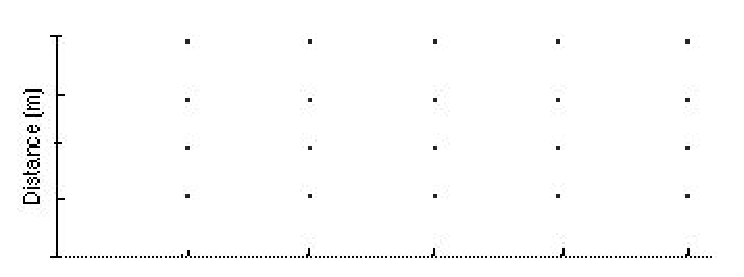
\includegraphics[width=4in]{periodic_motion/periodic_motion_fig2.eps}
%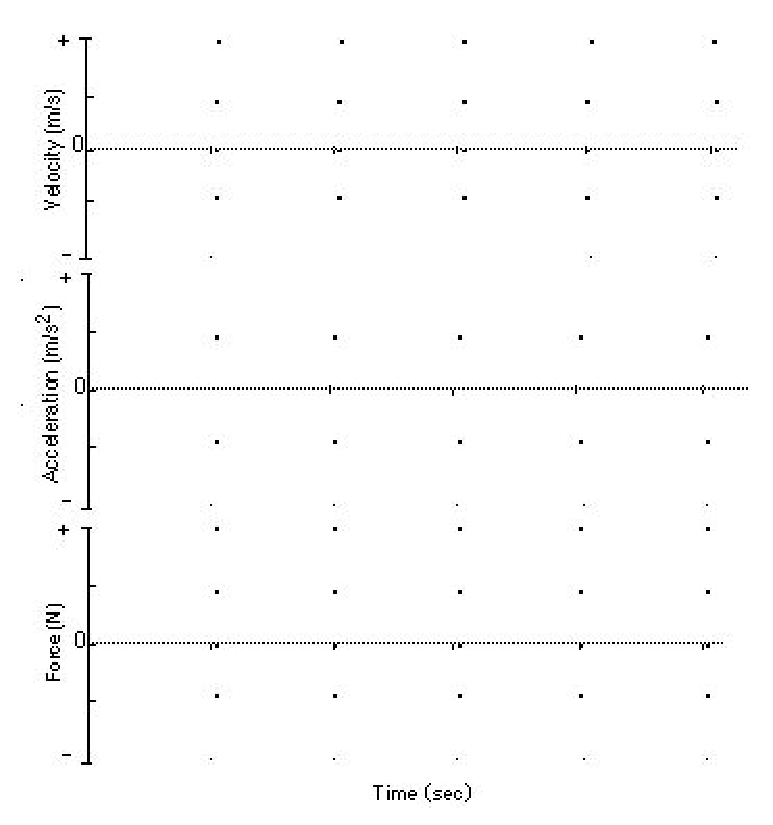
\includegraphics[width=4in]{periodic_motion/periodic_motion_fig3.eps}
%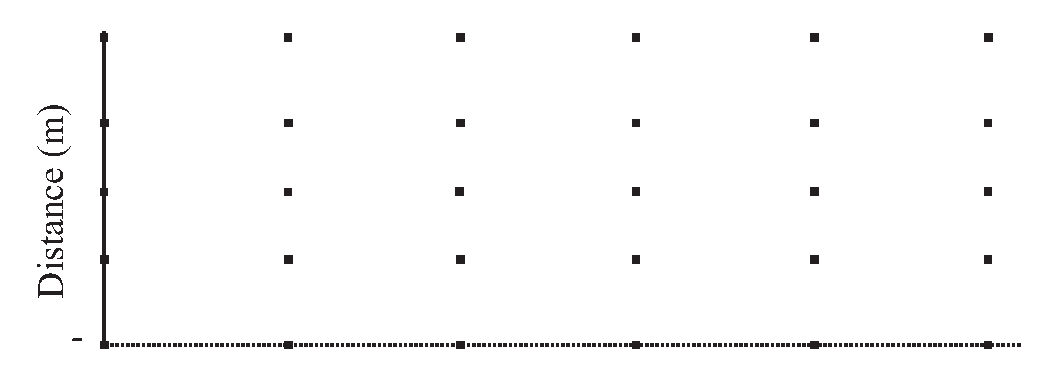
\includegraphics[width=4in]{periodic_motion/periodic_motion_fig2_new.eps}
%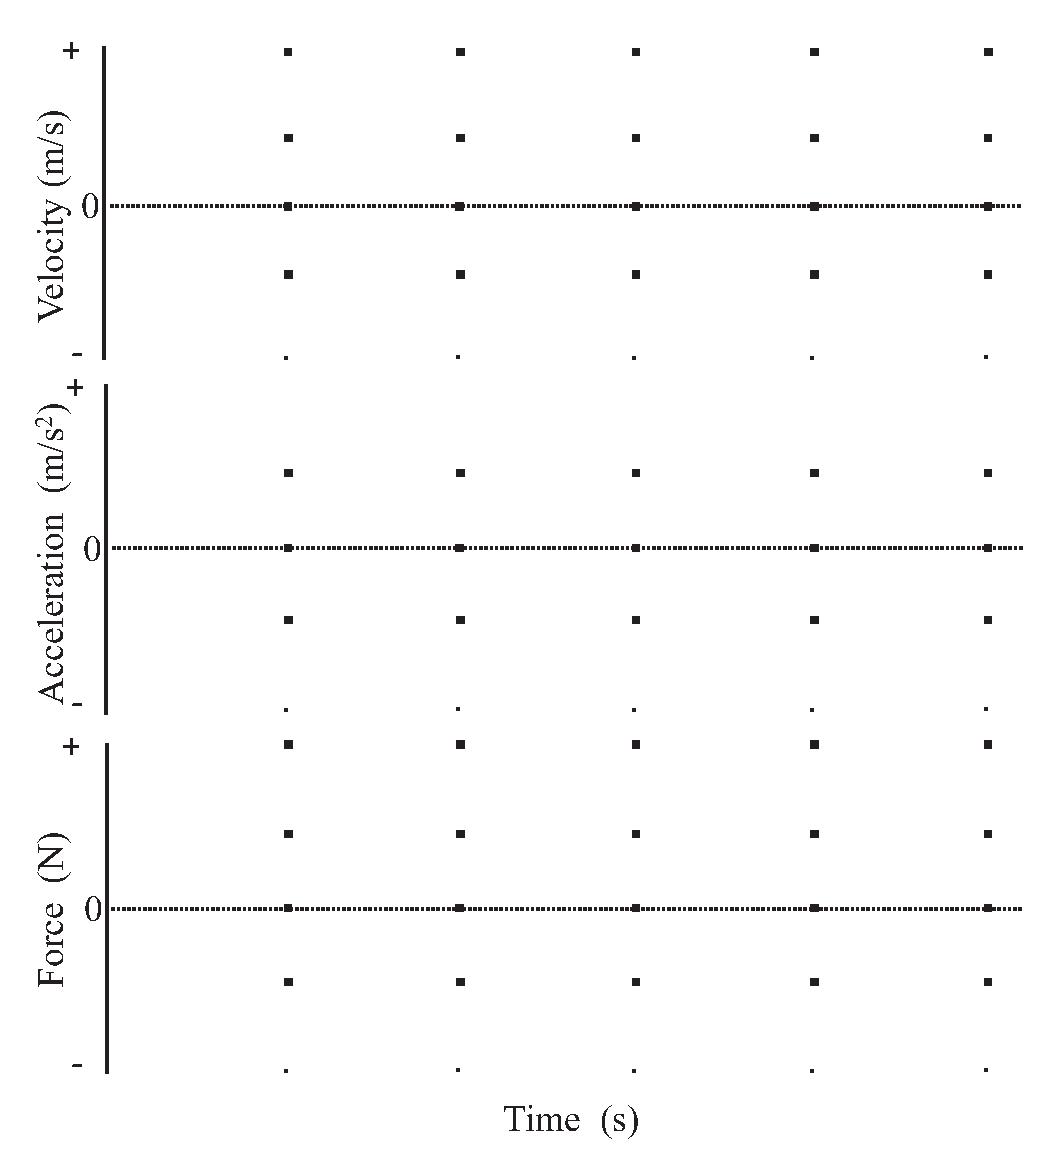
\includegraphics[width=4in]{periodic_motion/periodic_motion_fig3_new.eps}
%\end{center}

\begin{lab_groupplot}*{}[lab_grid,
	group style={
		group size=1 by 4,
		xlabels at=edge bottom,
		vertical sep=0.3in,
		},
	width=4.2in,  height=1.4in,
	xlabel=Time (s),
	xmin=0, xmax=3,
	xtick distance = 1, 
	ytick distance = 1, 
	minor x tick num=3,
	minor y tick num=1,
	ytick = {-1,0,1},
	yticklabels = {$-$, 0, $+$},
	]
\nextgroupplot[
	ytick distance = 1, 
	minor y tick num=3,
	ymin=0,ymax=1, 
	ylabel={Position (m)},
	]
\nextgroupplot[
	ymin=-1,ymax=1, 
	ylabel={Velocity (m/s)},
	]
\nextgroupplot[
	ymin=-1,ymax=1, 
	ylabel={Acceleration (m/s$^2$)},
	]
\nextgroupplot[
	ymin=-1,ymax=1, 
	ylabel={Force (N)},
	]
\end{lab_groupplot}

(b) Based on what you know about the relationships between velocity, 
acceleration, and force, use dashed lines to sketch your predictions for the 
acceleration and force graphs.

%(c) Suspend the 200-g mass from the spring and open the file \filename{SHM.cap} in the \filename{\coursefolder} folder. Calibrate the force probe (see Appendix~\ref{capstone}). Start the mass oscillating with an amplitude of 10~cm and record data for a few seconds. When you have obtained good graphs, sketch the results on the above axes using solid lines. Print your graph and attach to this unit.

(c) Open the file \filename{SHM.cap} in the \filename{\coursefolder} folder. Turn on the motion and force sensors at your station and connect them to the computer via Bluetooth. Tare the force sensor with noe applied force on the sensor's hook. Hang the large spring from the force sensor's hook with the large diameter coils down and hang a 200-g mass from the spring.  Place the motion sensor facing up directly below the spring. Start the mass oscillating with an amplitude of 10~cm and record data for a few seconds. When you have obtained good graphs, sketch the results on the above axes using solid lines. Print your graph and attach to this unit.

(d) When the mass is at its maximum distance from the motion sensor, is the absolute value of the velocity maximum, minimum or some other value according to your graphs? Does this agree
with your predictions? Does this agree with your observations of the oscillating
mass? Explain.
\answerspace{15mm}

\pagebreak[2]
(e) When the mass has its maximum positive velocity, is its distance from the
motion sensor maximum, minimum, the equilibrium value or some other value according
to your graphs? What about when it reaches maximum negative velocity? Does this
agree with your predictions? Does this agree with your observations of the 
oscillating mass? Explain. 
\answerspace{10mm}

(f) According to your graphs, for what distances from the motion sensor is the 
acceleration maximum? For what distances is the acceleration zero? What is the 
velocity in each of these cases?
\answerspace{20mm}

(g) Compare the force and acceleration-time graphs. Describe any similarities.
Does the force graph agree with your prediction?
\answerspace{20mm}

(h) From your graphs, what would you say is the relationship between force and
acceleration? 
\answerspace{20mm}

(i) Compare the force and distance(position)-time graphs. What would you say
is the relationship between force and position? 
\answerspace{20mm}

\textbf{Activity 5: Energy of a Mass Undergoing SHM }

Now use the graphs from Activity 1 to examine the energy relationships
in simple harmonic motion. To do this you will need to print the graphs and draw a horizontal line through the equilibrium position on the position vs. time graph.  
The $x$ values must be determined relative to this equilibrium position (which represents a displacement of zero).

(a) At what points is the kinetic energy of the mass zero? Label these points
on your distance and velocity graphs above with ``$K=0$''.

\pagebreak[2]
(b) Calculate the elastic potential energy due to the spring at one of these
points. Label the point you use on your velocity and distance graphs with a
1. Use $U = \frac{1}{2}kx^{2}$, where  $x$ is the distance from the equilibrium 
position and $k$ is the force constant of the spring, which you have already 
measured. Use the \textbf{Delta Tool} in the menubar (see Appendix {\it A})
to measure position, then subtract the 
equilibrium position to determine $x$. Show your data and calculations 
in the space below. 
\answerspace{20mm}

(c) At what points is the potential energy zero? Label these points with a ``$U=0$''
on your distance and velocity graphs.

(d) If you measured the kinetic energy at one of these points, what would you
expect its value to be? Explain.
\answerspace{15mm}

\pagebreak[2]
(e) Check your prediction. Calculate the kinetic energy at one of these points.
Label the point you use on your velocity graph with a 2. Use 
$K = \frac{1}{2} mv^{2}$, where $m$ is the total mass including half the mass of 
the spring. Use the \button{Delta Tool} to determine $v$. Show your data and 
calculations in the space below.
\answerspace{20mm}

(f) Did your calculated kinetic energy agree with your prediction?
\answerspace{15mm}

(g) If you calculated the potential and kinetic energies at a point where 
neither of these was zero, what would you expect the total energy to be? 
Explain.
\answerspace{20mm}

\pagebreak[3]
(h) Check your prediction. Make a table below with headings for $v$~(m/s), 
position ($m$), $x$~(m) where $x$ is the difference between the position
of the mass and the equilibrium position, $K$, $U$, and the total energy.
Pick 5 or 6 points where the mass has both kinetic and
potential energy, calculate them both ($K$ and $U$), and then calculate the 
total energy for each point ($K+U$). Label these points on your distance
and velocity graphs with numbers. 
Make a histogram of your results for the total energy and calculate the 
average and standard deviation.
For information on making histograms, see Appendix \ref{excel}. For information 
on calculating the average and standard deviation, see Appendix \ref{treatment}. 
Record the average and standard deviation here.
Attach the histogram to this unit.
\answerspace{80mm}

(i) What does the histogram of the total energy tell you? Be quantitative in 
your answer.
\answerspace{20mm}

(j) Is the total energy conserved?  Be quantitative in your answer.
\answerspace{20mm}

